%Notes by Harsh Mistry 
%CS 349
%Based on Template From  https://www.cs.cmu.edu/~ggordon/10725-F12/template.tex

\documentclass[twoside]{article}
\setlength{\oddsidemargin}{0.25 in}
\setlength{\evensidemargin}{-0.25 in}
\setlength{\topmargin}{-0.6 in}
\setlength{\textwidth}{6.5 in}
\setlength{\textheight}{8.5 in}
\setlength{\headsep}{0.75 in}
\setlength{\parindent}{0 in}
\setlength{\parskip}{0.1 in}
\usepackage{amsmath,amsfonts,graphicx}
\newcounter{lecnum}
\renewcommand{\thepage}{\thelecnum-\arabic{page}}
\renewcommand{\thesection}{\thelecnum.\arabic{section}}
\renewcommand{\theequation}{\thelecnum.\arabic{equation}}
\renewcommand{\thefigure}{\thelecnum.\arabic{figure}}
\renewcommand{\thetable}{\thelecnum.\arabic{table}}
\newcommand{\lecture}[4]{
   \pagestyle{myheadings}
   \thispagestyle{plain}
   \newpage
   \setcounter{lecnum}{#1}
   \setcounter{page}{1}
   
   
%Info Box 
   \begin{center}
   \framebox{
      \vbox{\vspace{2mm}
    \hbox to 6.28in { {\bf CS 349 - User Interfaces
	\hfill Winter 2018} }
       \vspace{4mm}
       \hbox to 6.28in { {\Large \hfill Lecture #1: #2  \hfill} }
       \vspace{2mm}
       \hbox to 6.28in { {\it Lecturer: #3 \hfill Notes By: #4} }
      \vspace{2mm}}
   }
   \end{center}
   
   \markboth{Lecture #1: #2}{Lecture #1: #2}



 
}

\renewcommand{\cite}[1]{[#1]}
\def\beginrefs{\begin{list}%
        {[\arabic{equation}]}{\usecounter{equation}
         \setlength{\leftmargin}{2.0truecm}\setlength{\labelsep}{0.4truecm}%
         \setlength{\labelwidth}{1.6truecm}}}
\def\endrefs{\end{list}}
\def\bibentry#1{\item[\hbox{[#1]}]}

\newcommand{\fig}[3]{
			\vspace{#2}
			\begin{center}
			Figure \thelecnum.#1:~#3
			\end{center}
	}
	
\graphicspath{ {images/} }

\newtheorem{theorem}{Theorem}[lecnum]
\newtheorem{lemma}[theorem]{Lemma}
\newtheorem{ex}[theorem]{Example}
\newtheorem{proposition}[theorem]{Proposition}
\newtheorem{claim}[theorem]{Claim}
\newtheorem{corollary}[theorem]{Corollary}
\newtheorem{definition}[theorem]{Definition}
\newenvironment{proof}{{\bf Proof:}}{\hfill\rule{2mm}{2mm}}
\newcommand\E{\mathbb{E}}


%Start of Document 
\begin{document}

\lecture{9}{January 24, 2018}{Keiko Katsuragawa}{Harsh Mistry}

\section{Event Binding}
Event binding answers how we bind an event event to code after dispatch to a widget

\subsection{Event-to-Code Binding Approaches}
\begin{itemize}
\item Event loop + Switch statement "manual" binding
\item Switch statement binding
\item Inheritance binding
\item Listener interface binding 
\item Listener object binding
\item Listener adapter binding. 
\item Delegate binding (C\#)
\end{itemize}

\subsubsection{Event Loop and Switch Statement Binding}
\begin{itemize}
\item All events consumed in one event loop (not by widgets) 
\item Switch selects window and code to handle the event
\item Used in Xlib and many early systems
\end{itemize}

\begin{center}
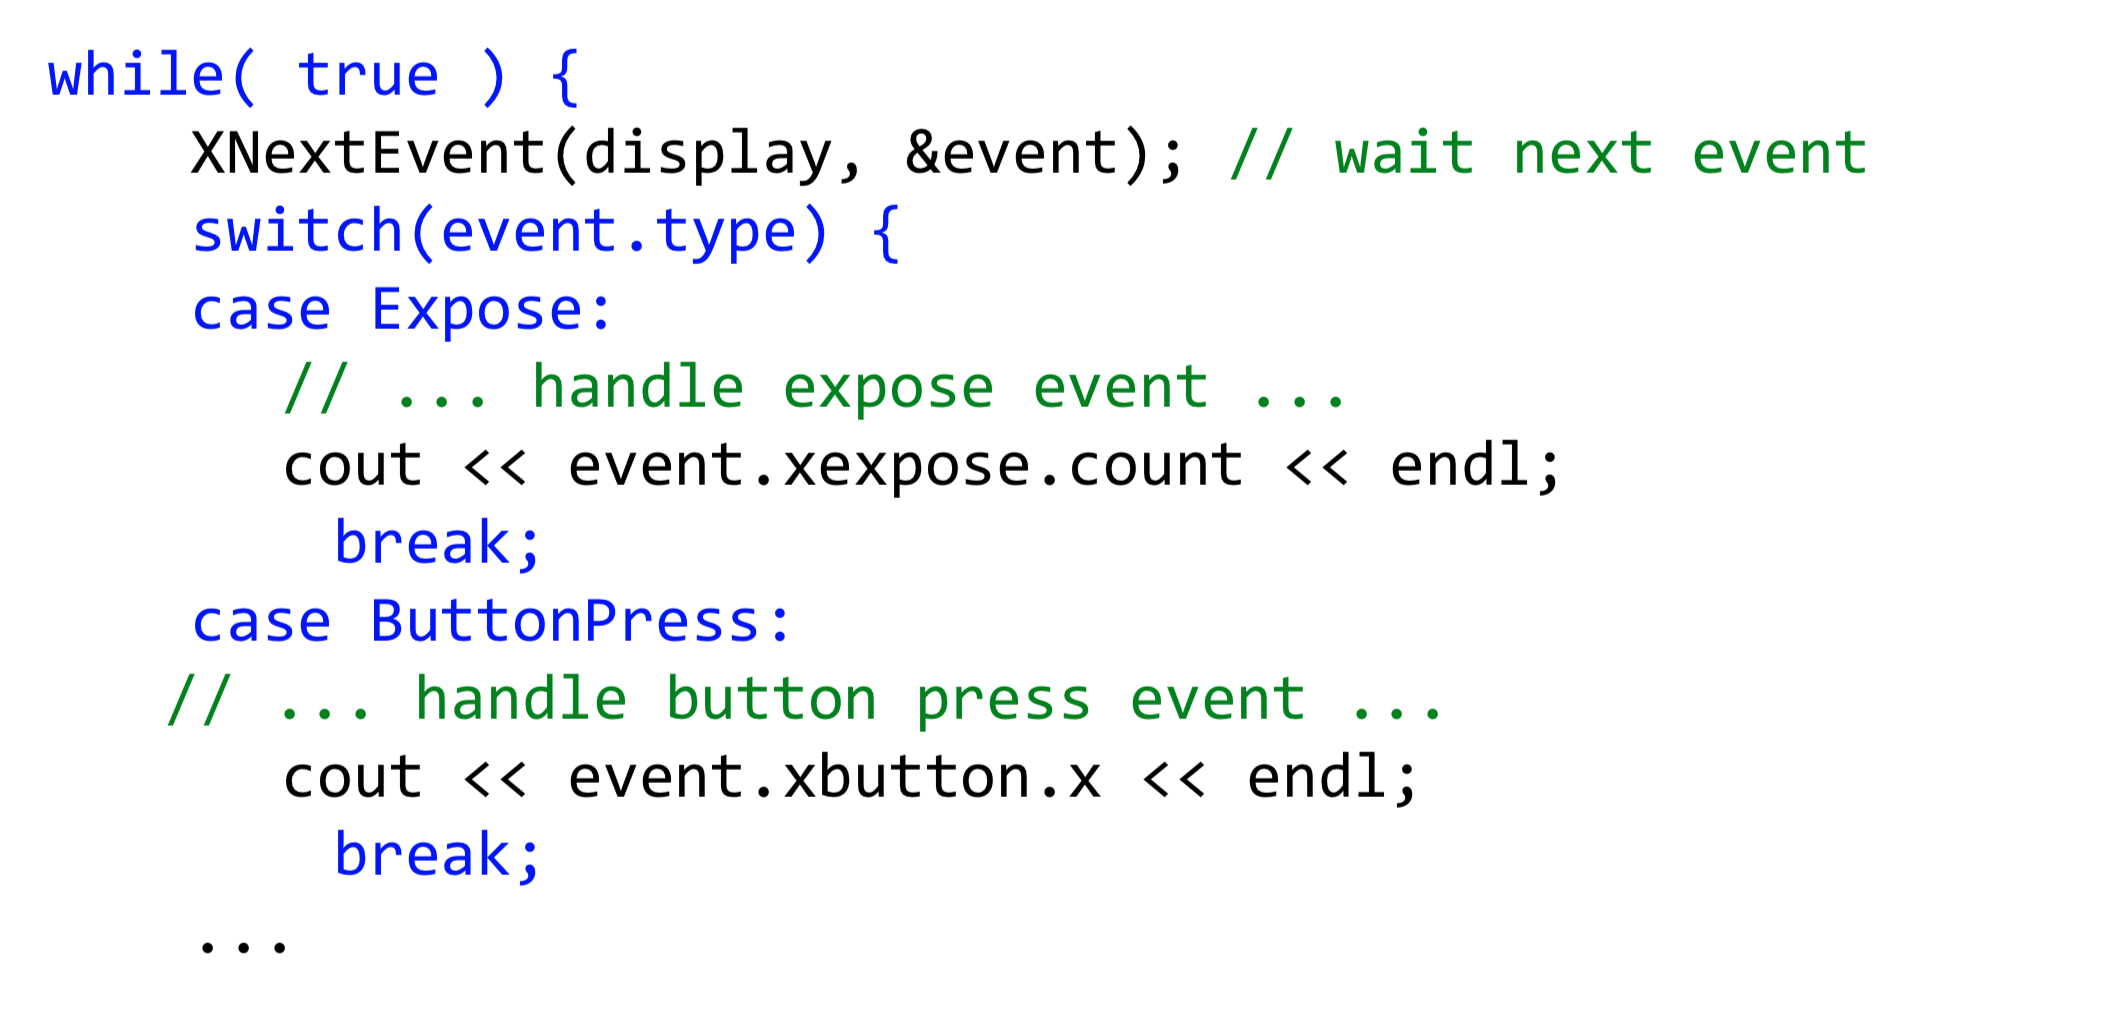
\includegraphics[scale=0.2]{26}\\
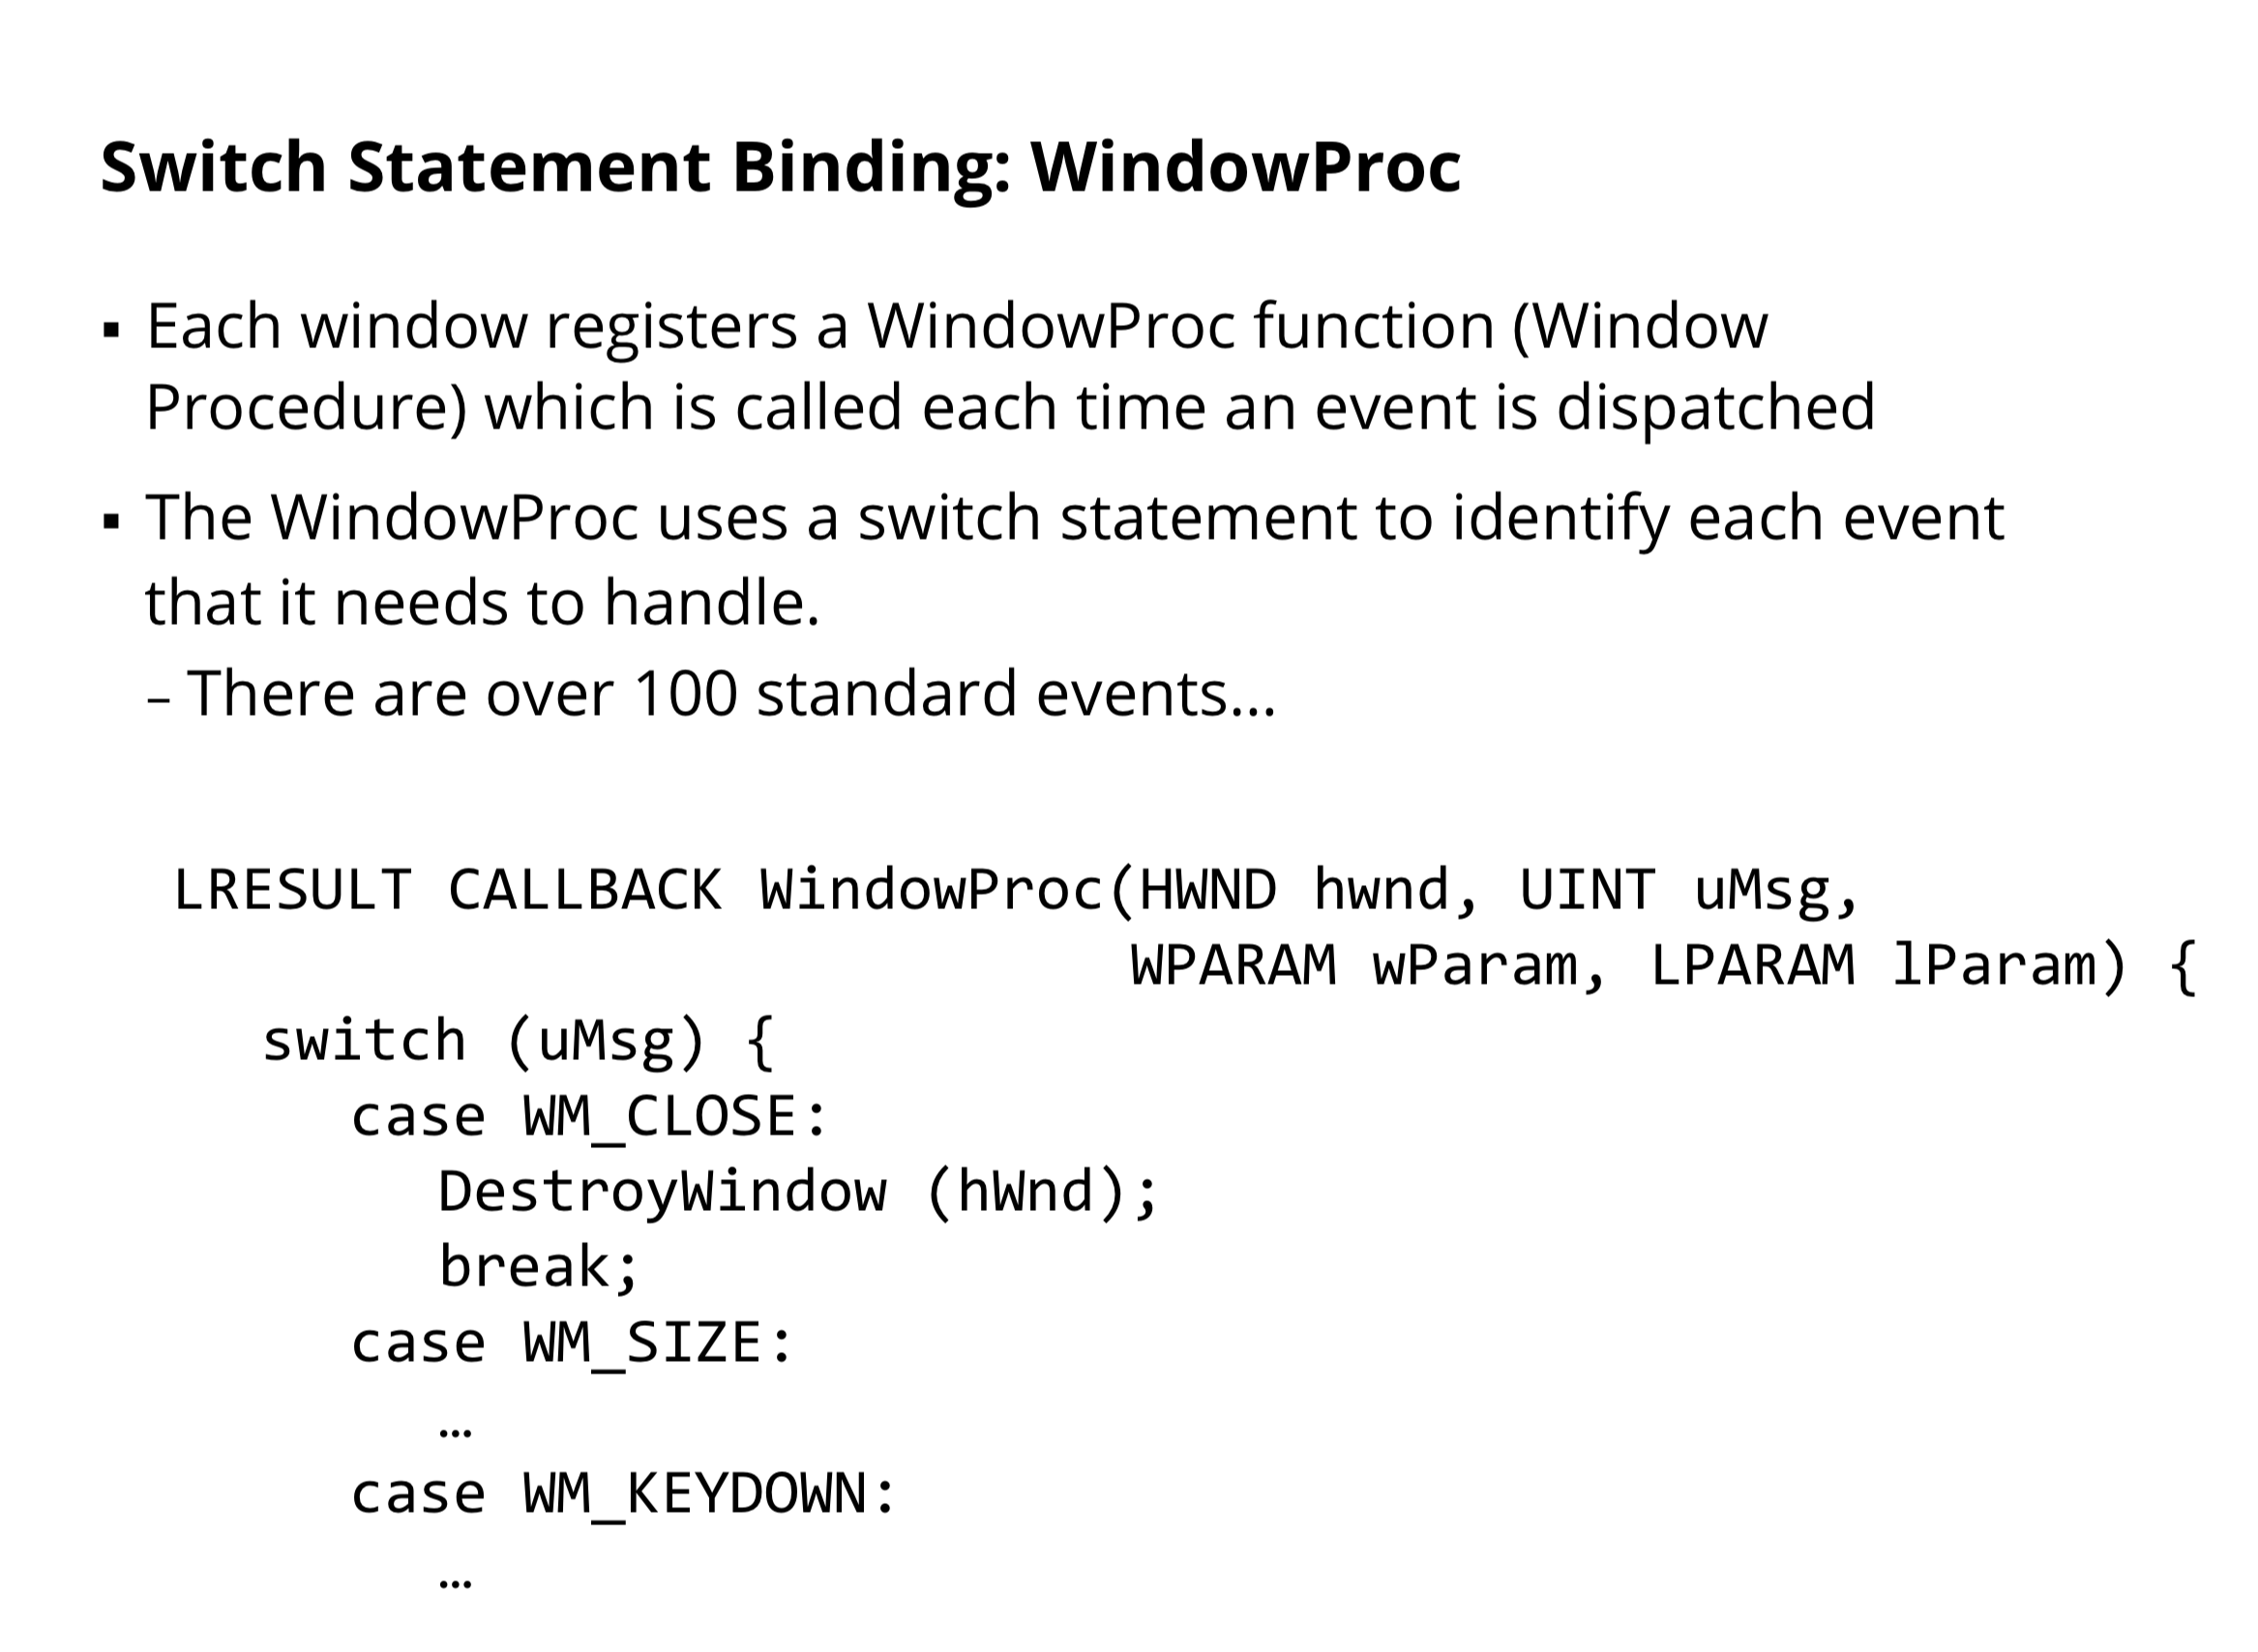
\includegraphics[scale=0.25]{27}
\end{center}

\subsubsection{Inheritance Binding}
\begin{itemize}
\item Event is dispatched to an Object-Oriented (OO) widget
\item OO widget inherits from a base widget class with all event
handling methods defined a priori onMousePress, onMouseMove, onKeyPress, etc
\item The widget overrides methods for events it wishes to handle -  Each method handles multiple related events
\item Used in Java 1.0
\end{itemize}

\subsubsection{Inheritance Problems}
\begin{itemize}
\item Each widget handles its own events, or the widget container has to check what widget the event is meant for
\item Multiple event types are processed through each event method -  complex and error-prone, just a switch statement again
\item No filtering of events: performance issues
\item It doesn’t scale well: How to add new events? -  e.g. penButtonPress, touchGesture, ....
\item Muddies separation between GUI and application logic: event handling application code is in the inherited widget
\item Use inheritance for extending functionality, not binding events

\end{itemize}
\subsubsection{Delegate Binding}
\begin{itemize}
 \item Interface architecture can be a bit heavyweight
\item Can instead have something closer to a simple function callback (a
function called when a specific event occurs)
\item Delegates in Microsoft’s .NET are like a C/C++ function pointer for methods, but they: \\
-  Are object oriented\\
-  Are completely type checked\\
-  Are more secure
-  Support multicasting (able to “point” to more than one method)\\
\item  Using delegates is a way to broadcast and subscribe to events
\item .NET has special delegates called “events”
\end{itemize}

\begin{center}
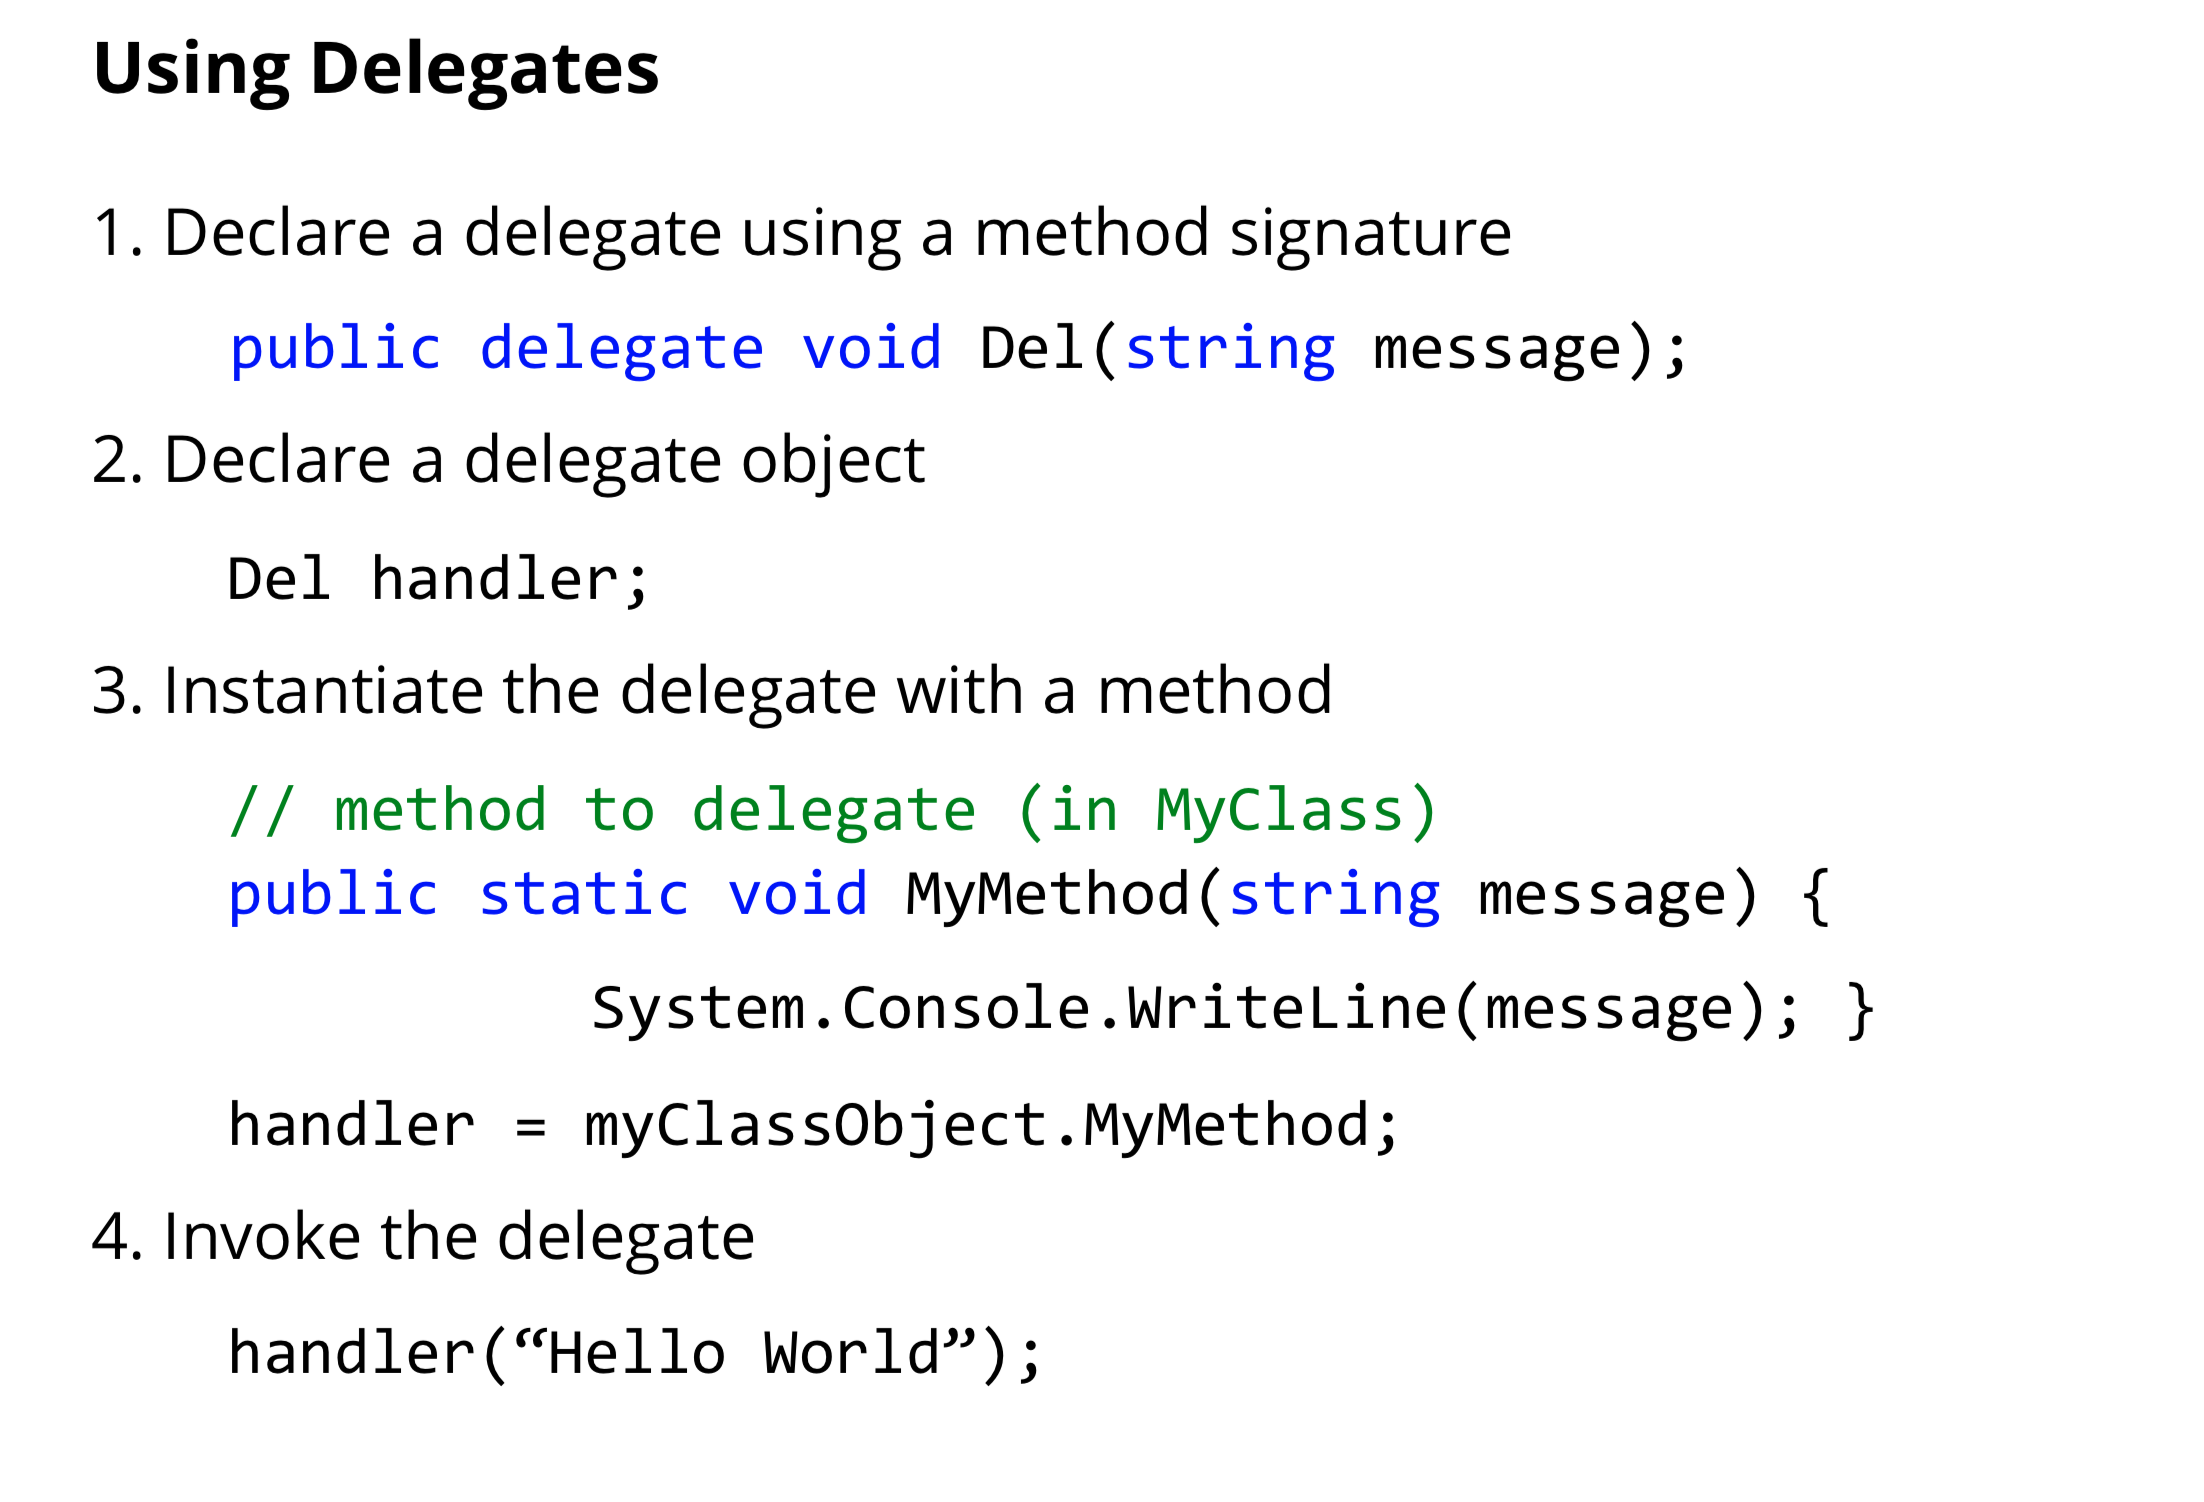
\includegraphics[scale=0.2]{28}\\
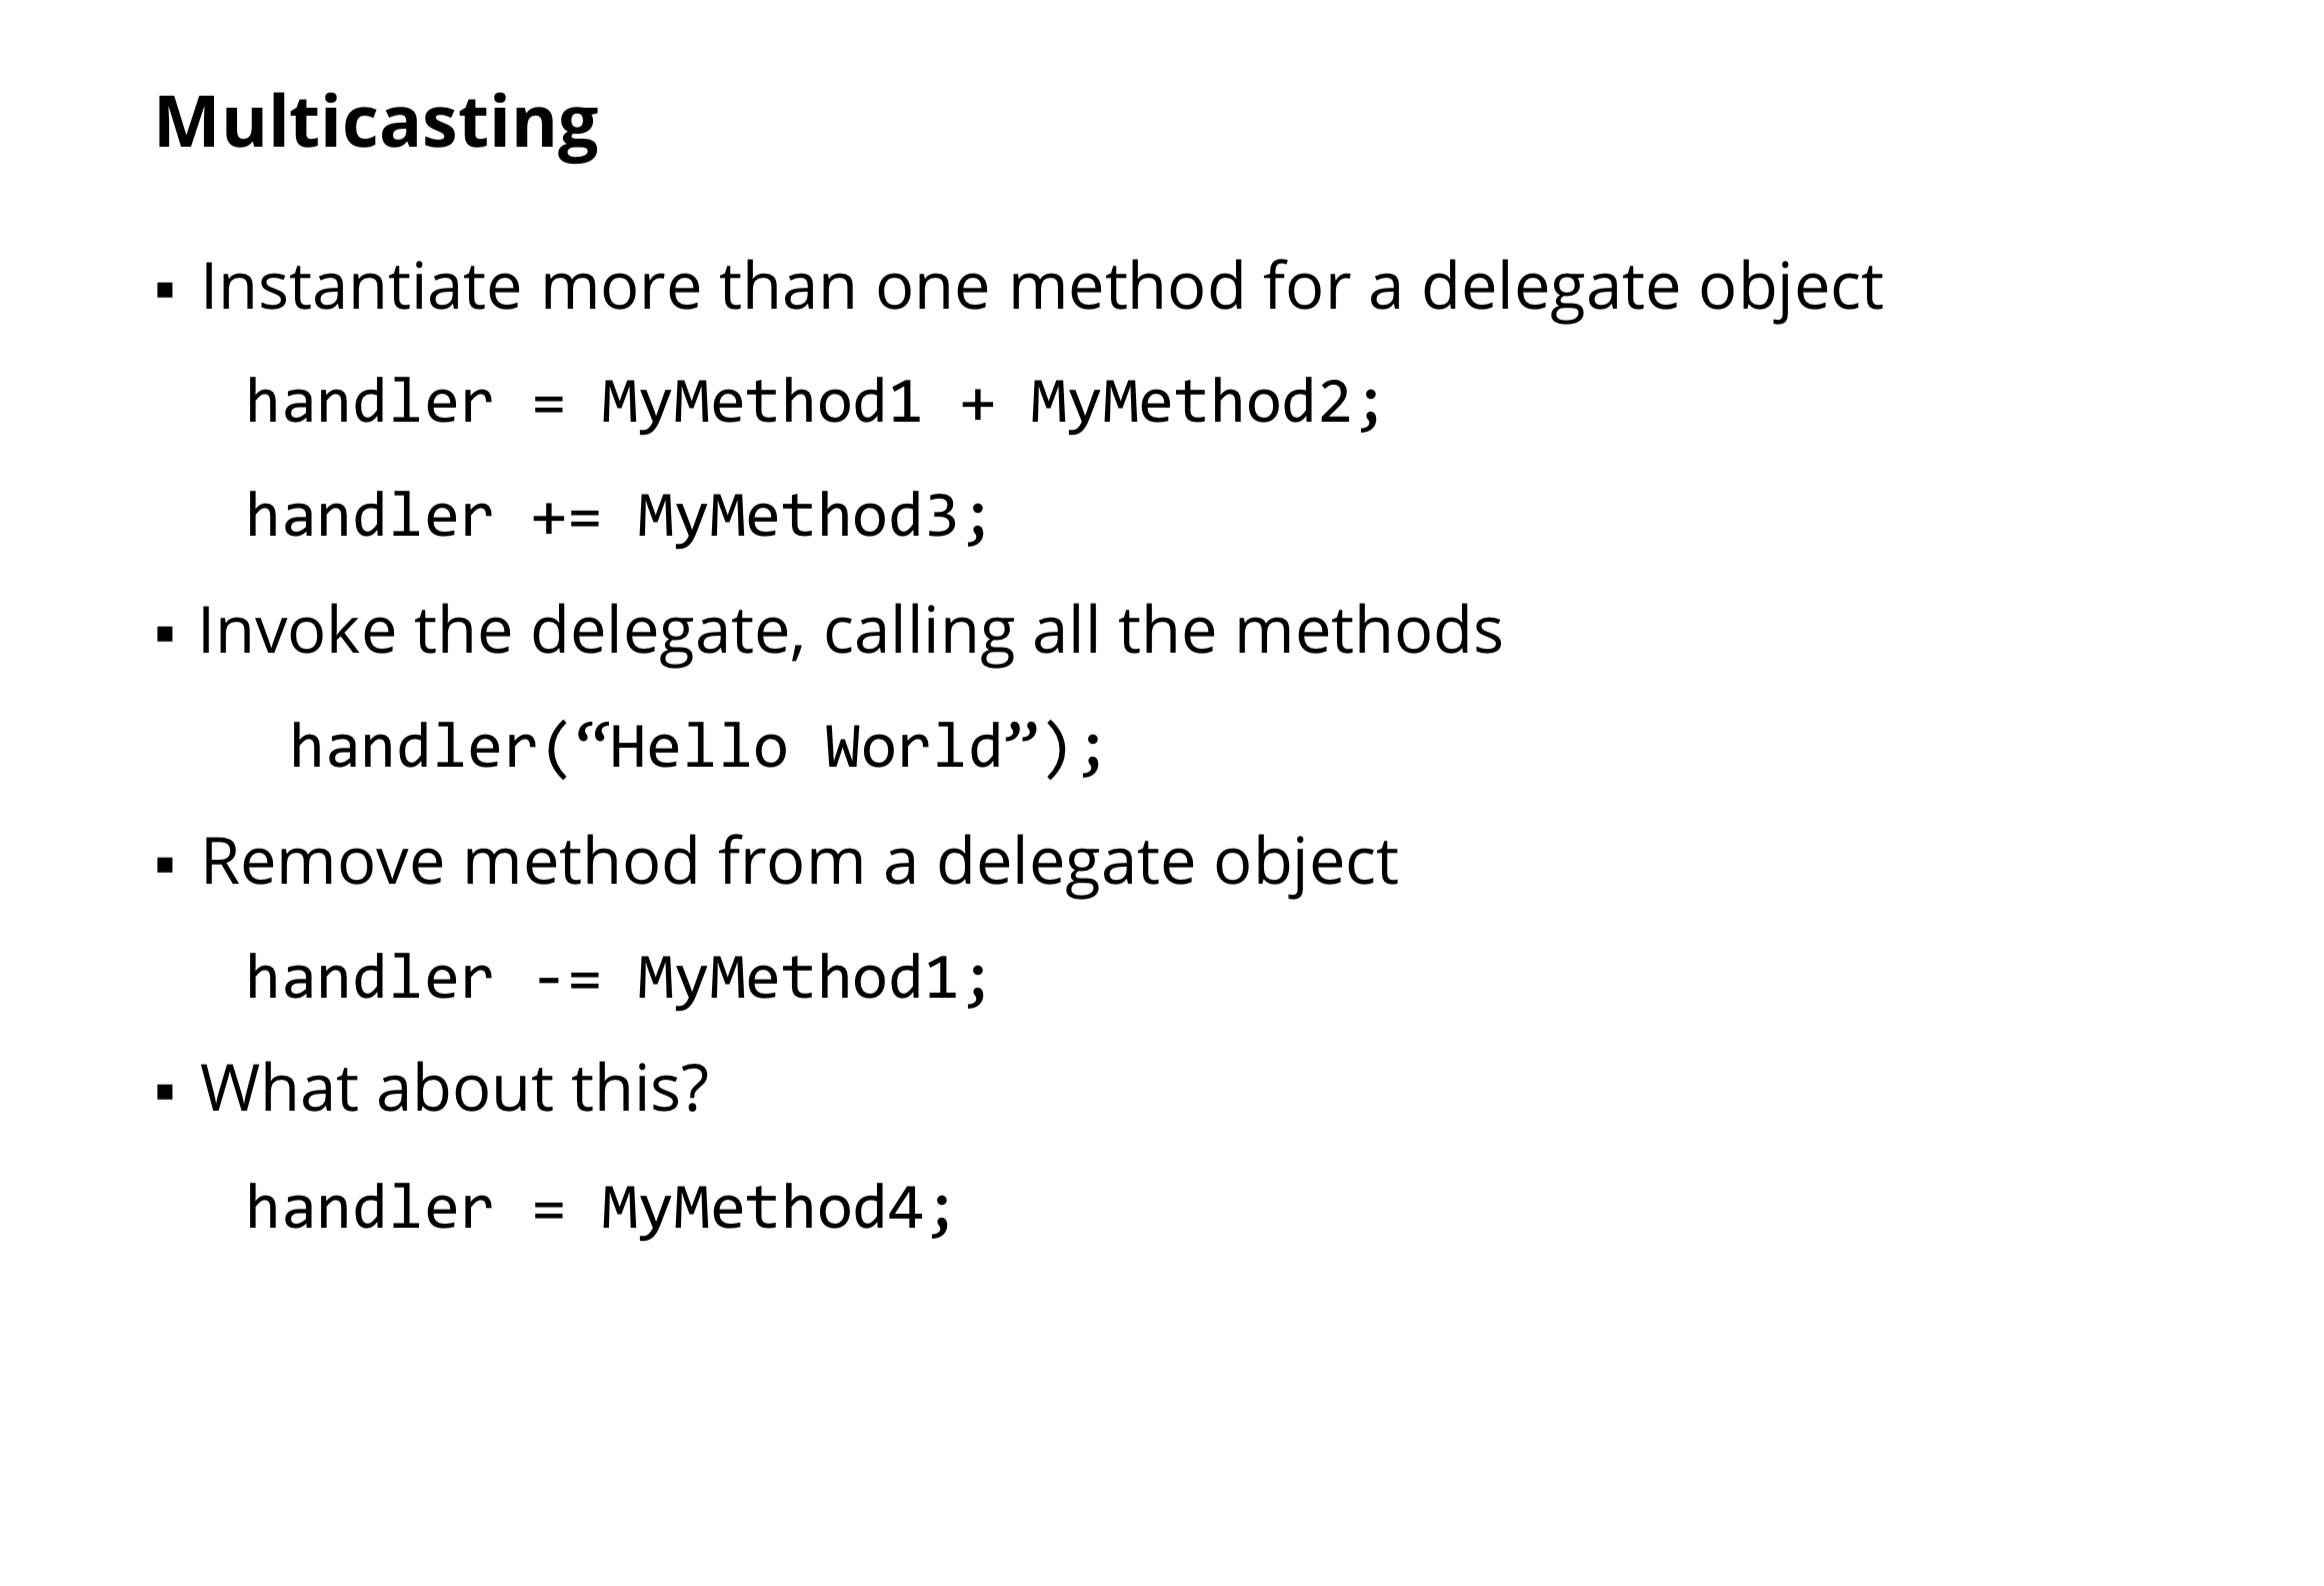
\includegraphics[scale=0.2]{29}\\
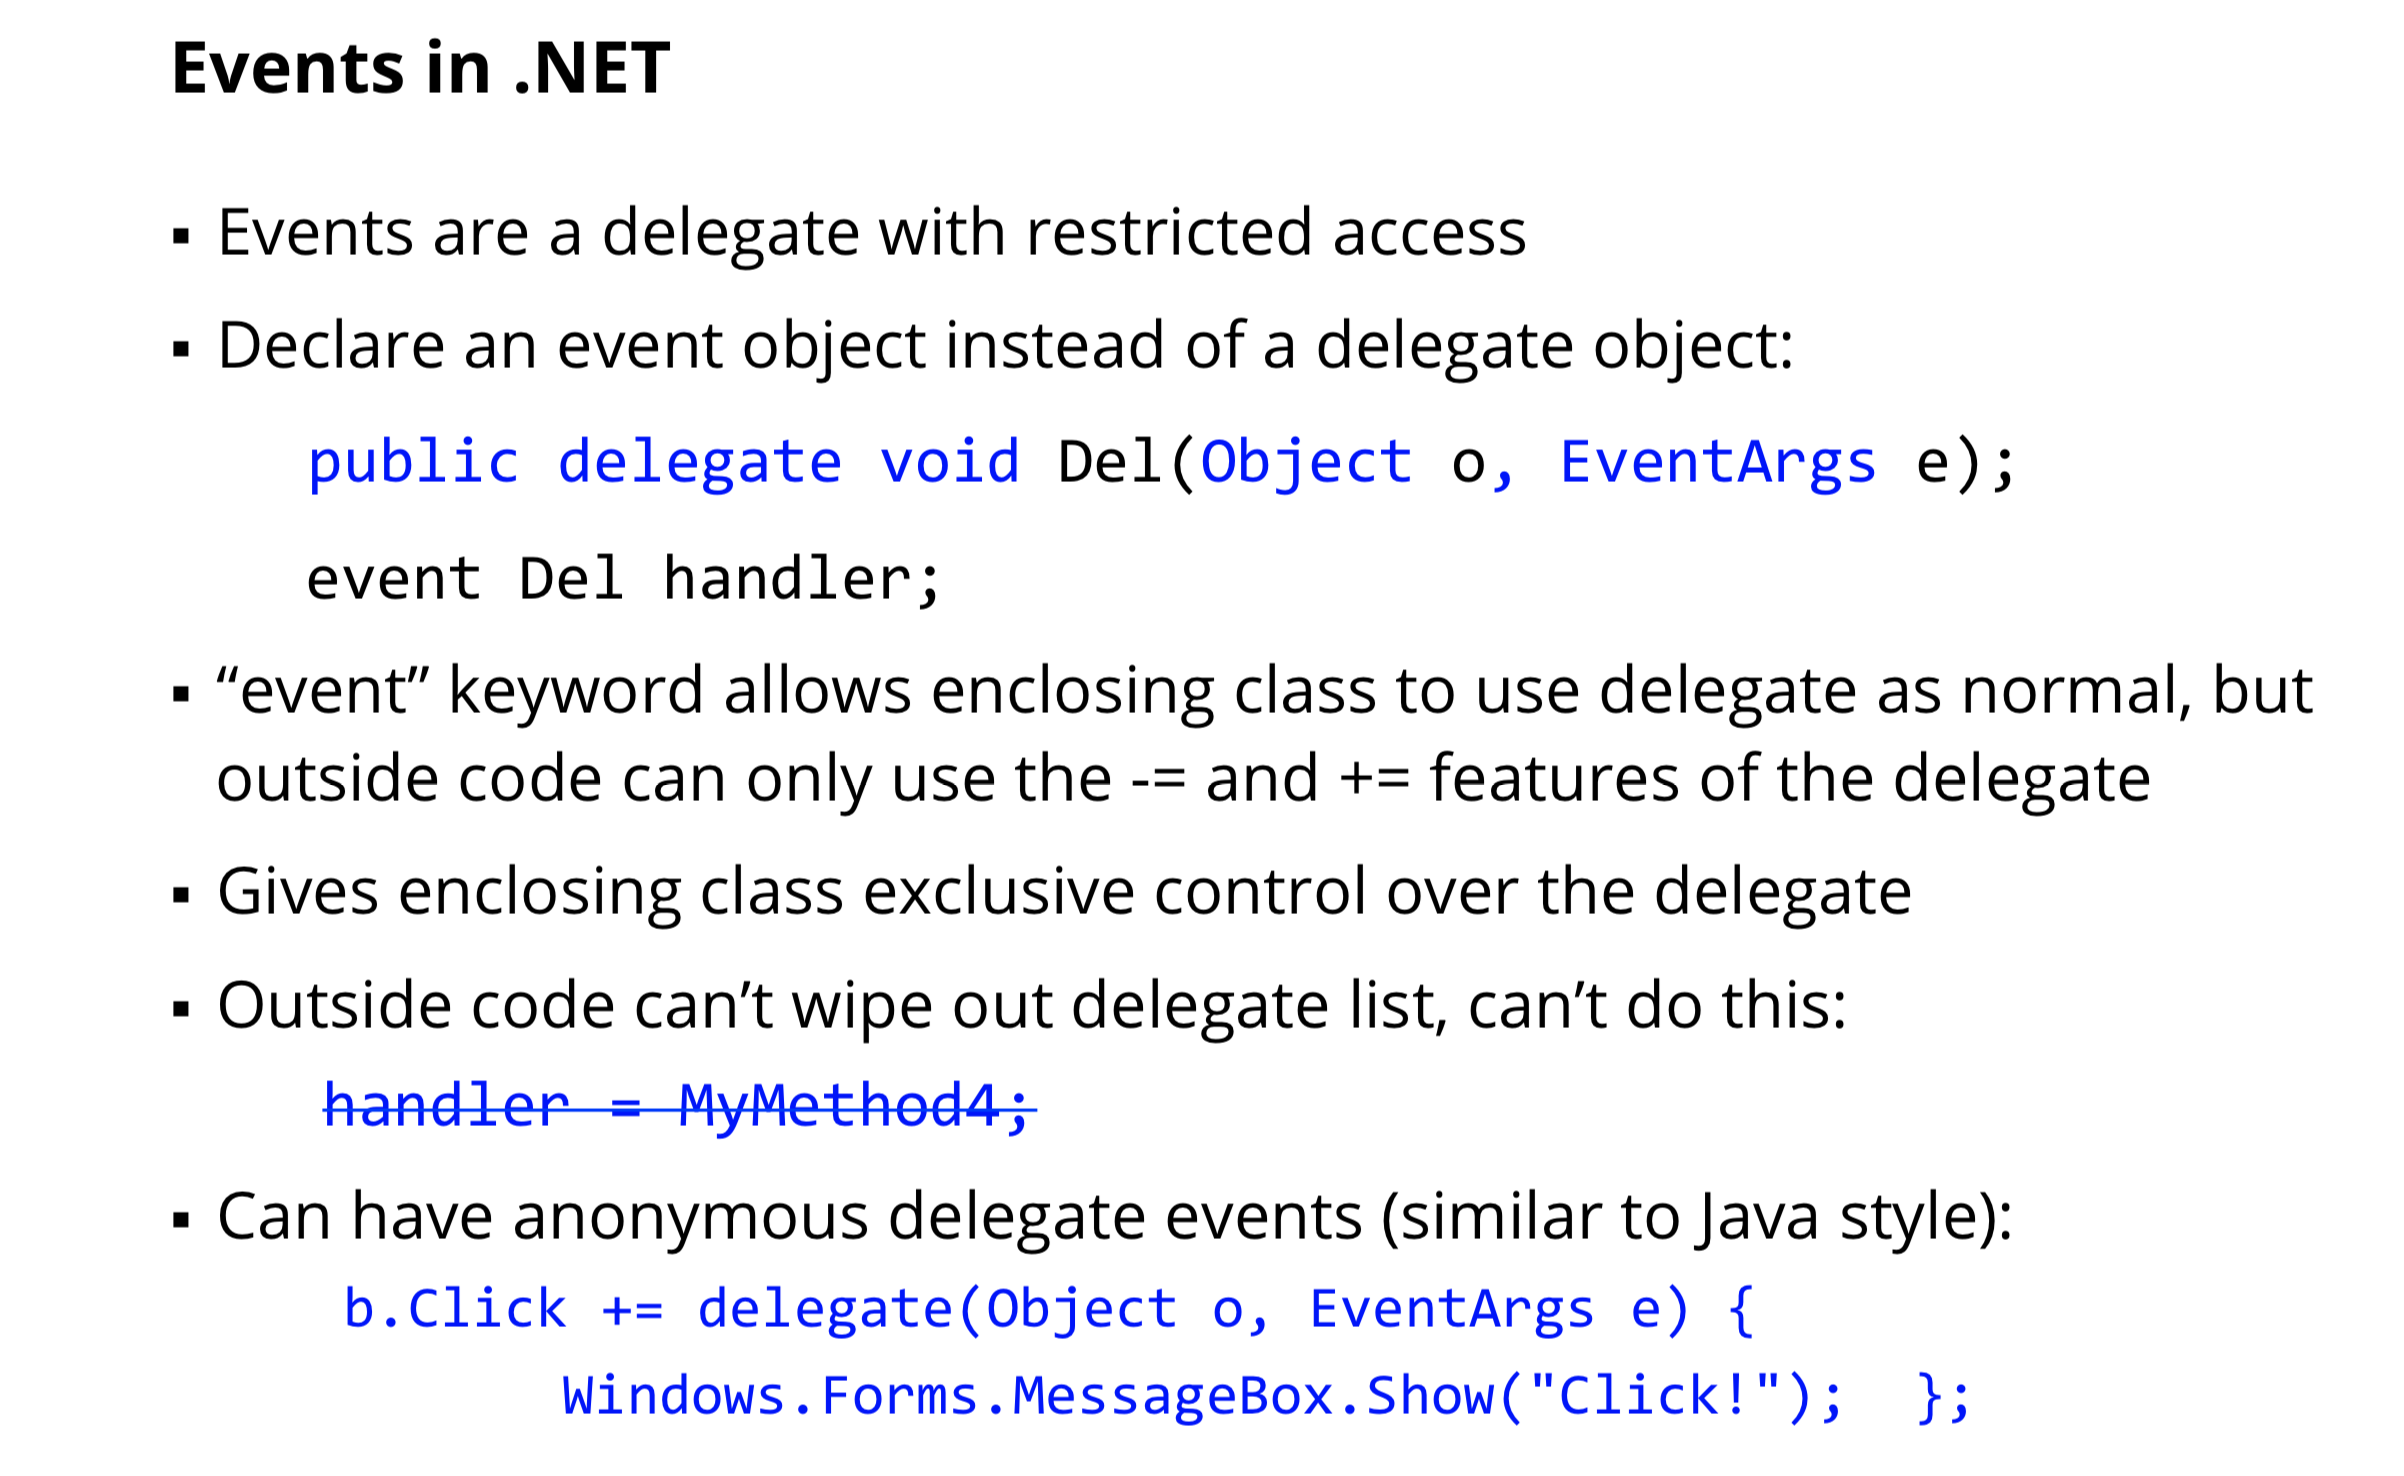
\includegraphics[scale=0.2]{30}
\end{center}

\end{document}





